% A workaround to allow relative paths in included subfiles
% that are to be compiled separately
% See https://tex.stackexchange.com/questions/153312/subfiles-inside-a-subfile-using-relative-paths
\providecommand{\main}{..}
\documentclass[\main/thesis.tex]{subfiles}

\begin{document}

\chapter{Matrix Multiplication}
\label{cha:matmul}
Matrix multiplication has long been intrinsic to the \gls{hpc} communities, be it the general scientific community or within the computing science domain.
Several fields within physics~\autocite{krol2014matrix}, biology~\autocite{akutsu2000algorithms} and chemistry~\autocite{weber2015semiempirical} all benefit from matrix multiplication in some way.
It is also possible to simulate quantum computing processes using matrix multiplication~\autocite{zulehner2019matrix}.
Beyond this, it is well known that many neural-network operations are based on matrix-matrix or vector-matrix multiplication~\autocite{rojas1996neural,blue1992training}.

Due to its simple structure, tight loop layout, but potentially long execution time, matrix multiplication is well positioned to be improved in both software and hardware.
Seminal research such as that by Goto and van de Geijn~\autocite{goto2008anatomy} has resulted in high performance software implementations like EIGEN~\autocite{guennebaud2021eigen} and OpenBLAS~\autocite{xianyi2012model}.
These implementations often outperform na\"ive versions of matrix multiplication by hundreds or thousands of times, turning hours of serial work into seconds or less.
This speedup is possible through the use of hardware features, such as \gls{simd}, and software optimisations, such as loop blocking and data packing.
Understanding matrix multiplication and how it is implemented is critical to unlocking these optimisations.

\section{Inner and Outer Product}
\label{sec:products}
\bk{
  Should the code in this section be algorithms instead of listings?
  I think ``listings'' are meant to formatted output, e.g. printed output or resulting IR.
  ``Algorithms'' are processes to get output.
  That being said, algorithms might instead be seen as ``this is a contribution'' and listings could be ``less important code that must still be typeset nicely''.
}
Computing matrix multiplication, as taught in an introductory math course, is performed using what is known as the \emph{inner product}.
This is not to be confused with the \emph{dot product}, which is an operation between vectors and is used when computing the inner product, or \emph{outer product}, which is a different method of computing matrix multiplication like the inner product.
Both the outer product and inner product compute the same output given the same input but, as \rsec{outerKernel} and \rsec{innerKernel} will discuss, the efficacy with which they arrive at the destination can vary greatly.

\begin{figure}[t]
 \hfill
  \begin{subfigure}{.45\linewidth}
    \centering
    \begin{tikzpicture}[scale=1/2]
      \draw[step=1, shift={(0, 3)}] (0, 0) grid +(4, 1);
      \node at (4.75, 2) {$\times$};
      \draw[step=1, shift={(5.5, 0)}] (0, 0) grid +(1, 4);
      \node at (7.25, 2) {$=$};
      \draw[step=1, shift={(8, 3)}] (0, 0) grid +(1, 1);
      \node at (2, 5) {$A$};
      \node at (6, 5) {$B$};
      \node at (8.5, 5) {$C$};
    \end{tikzpicture}
    \caption{Inner product.}
    \label{fig:innerProduct}
  \end{subfigure}
 \hfill
  \begin{subfigure}{.45\linewidth}
    \centering
    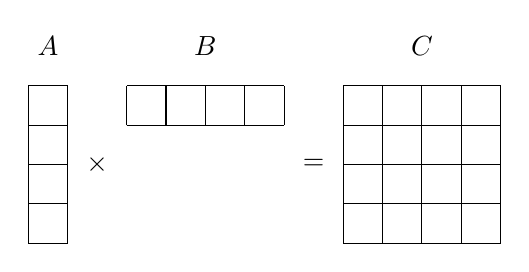
\begin{tikzpicture}[scale=1/2]
      \draw[step=1, shift={(0, 0)}] (0, 0) grid +(1, 4);
      \node at (1.75, 2) {$\times$};
      \draw[step=1, shift={(2.5, 3)}] (0, 0) grid +(4, 1);
      \node at (7.25, 2) {$=$};
      \draw[step=1, shift={(8, 0)}] (0, 0) grid +(4, 4);
      \node at (.5, 5) {$A$};
      \node at (4.5, 5) {$B$};
      \node at (10, 5) {$C$};
    \end{tikzpicture}
  \caption{Outer product (rank-$1$ update).}
    \label{fig:outerProduct}
  \end{subfigure}
  \hfill
  \caption{Example matrix-matrix multiplication computation styles.}
  \label{fig:product}
  \vspace{-0.15cm}
\end{figure}

\subsection{The Inner Product}
Given the computation \matmul{M}{D}{N}, the inner product is computed by taking the dot product of the $i$th row of $A$ and the $j$th column of $B$ to produce the cell $c_{i,j}$ (\rfig{innerProduct}).
The dot product is defined as the summation of the pair-wise products of the two vectors (\eg $a_{i,1}b_{1,j} \times a_{i,2}b_{2,j} \times \ldots \times a_{i,D}b_{D,j}$).
Therefore, in its most naive form, matrix multiplication can be computed like so:
\begin{lstlisting}[caption={[Basic inner product]A basic matrix multiplication via inner product.},label=lst:basicInner,language=C++,columns=flexible,morekeywords=uint64_t]
for (uint64_t i = 0; i < M; ++i)
  for (uint64_t j = 0; j < N; ++j)
      for (uint64_t k = 0; k < D; ++k)
        C[i][j] += A[i][k] * B[k][j];
\end{lstlisting}
The \code{i} loop iterates the rows of $A$, also choosing a row in $C$, while the \code{j} loop iterates the columns of $B$, also choosing a cell in the chosen row of $C$.
The final \code{k} loop iterates through the elements of the chosen row of $A$ and column of $B$, computing the dot product by accumulating (reducing) each of the pair-wise products into the chosen cell of $C$.

\subsection{The Outer Product}
The outer product, when seen in mathematics, is typically seen only when $D=1$ as in \matmul{M}{1}{N}, mimicking the diagram in \rfig{outerProduct}.
Mathematicians prefer to view \matmul{M}{D}{N} with $D > 1$ as an inner product for simplicity, using the outer product only when $D=1$.

Given the same computation, \matmul{M}{D}{N}, the outer product is computed by multiplying a column of $A$ with a row of $B$ as in \rfig{outerProduct}, producing an output matrix.
Where, given a vector from $A$ and $B$, the inner product fully computes a single cell, the outer product partially computes every cell of the output $C$.
In its most na\"ive form, it appears as in \rlst{basicInner} but with the $k$ loop switched to be the outermost loop:
\begin{lstlisting}[caption={[Basic outer product]A basic matrix multiplication via outer product.},label=lst:basicOuter,language=C++,columns=flexible,morekeywords=uint64_t]
for (uint64_t k = 0; k < D; ++k)
  for (uint64_t i = 0; i < M; ++i)
    for (uint64_t j = 0; j < N; ++j)
        C[i][j] += A[i][k] * B[k][j];
\end{lstlisting}
Now, the $k$ loop chooses a pair of column from $A$ and row from $B$ that are iterated by the $i$ and $j$ loops respectively.
Rather than focusing on a single cell of $C$, every element of $C$ will be updated once before returning to the first cell with a new column and row combination.

\subsubsection{Rank-\texorpdfstring{$r$}{r} Updates}
Some mathematical operations, such as lower-upper factorization, depend on a changing data set, updating a model as new data points are added~\autocite{strange2007efficient}.
This update process is performed by taking a matrix derived from the model and updating it with the outer product of two vectors.
\bk{
  I say ``a matrix derived from the model'' because it's probably very out of the scope of this paper (and my knowledge at this point) on where this matrix comes from.
  I know enough to only make this next point about rank-1 update.
}
Because the result of the outer product of two vectors, a matrix, will always be of rank one\footnotemark, this is called a \emph{rank-one update}.
\footnotetext{All rows and columns are a linear combination of one vector. For example, given $M=xv^T$ all columns in $M$ are a multiple of $x$.}
Matrix multiplication can be computed in the same way by updating a zeroed-out matrix with outer products (the rank-one update), evenutally arriving at a fully computed multiplication: $C^1=0; C^{k+1}=C^k+A_{*,k}B_{k,*}$.
With this model, the outer product matrix multiplication in \rlst{basicOuter} is rewritten as such:
\begin{lstlisting}[caption={[Matrix multiplication via rank-one update]Matrix multiplication using rank-one update.},label=lst:rankOne,language=C++,columns=flexible,morekeywords=uint64_t]
for (uint64_t k = 0; k < D; ++k)
  rankOneUpdate(C, column(A, k), row(B, k));
\end{lstlisting}

It is not necessary for a complicated model to update itself one data point at a time.
Should, for example, two data points become simultaneously available, two rank-one updates can be performed at the same time.
Updating with two rank-one updates means summing two rank-one matrices; by definition, the summation of two rank-one matrices creates a rank two matrix\footnotemark.
\footnotetext{Given matrices $M_1, M_2 \in \mathcal{R}^{m \times n}$, each rank one, then each matrix has $v_i$, its only basis vector. If $v_1 \ne v_2$, then $M_1+M_2$ has two basis vectors $v_1, v_2$, implying $M_1+M_2$ has rank two.}
Therefore, this can now be described as a rank-two update.
This same logic extends to creating updates with greater ranks, giving rise to the rank-$r$ update\footnotemark.
\footnotetext{Common notation is rank-$k$ update; it is changed to rank-$r$ update in this work so as to avoid confusion with $k$ in other uses.}
Revisiting the process in \rlst{rankOne}, this repeated rank-one update process is apparent.
The loop simply performs $D$ rank-one updates, implying this can be once again reinterpreted in the form of one rank-$D$ update like so:
\begin{lstlisting}[caption={[Matrix multiplication via rank-$r$ update]Matrix multiplication using rank-$r$ update.},label=lst:rankR,language=C++,columns=flexible,morekeywords=uint64_t]
// Assumption: A, B are arrays of D vectors
rankRUpdate(C, A, B, /*rank*/ D);
\end{lstlisting}

\section{State of the Art}
Matrix multiplication, as a critical operation in many applications, has been the focus of optimisation research for decades.
Simple insights into matrix multiplication have enabled better data usage, both spatially and temporally.
Contemporary libraries and their overall frameworks are derived from seminal work by Goto and van de Geijn~\autocite{goto2008anatomy}.
More recent work~\autocite{vanzee2015blis,zee2016blis} have improved upon that seminal work, but the overall structure remains the same.
Each of these works aim to improve the portability to new architectures by providing a more modular approach for the micro kernel.
This includes a work by Low \etal which shows that the tuning parameters of the kernels for each architecture can be derived analytically from the architecture specification~\autocite{low2016analytical}.

Goto and van de Geijn's work concludes that matrix multiplication should be implemented in a \emph{layered approach}.
Each of these ``layers'' is typically one or more loops that perform some function before executing the enclosed layer.
It can be convenient to think of each of the upper layers as a function with a nested function call within it.
The innermost layer in this view performs the most basic computation on which the entire operation is built, essentially a small and fast matrix multiplication.
The surrounding layers are concerned with the optimisation of data movement and layout.

Typically, the layered approach consists of two layers:
\begin{enumerate*}[itemjoin={{; }}, itemjoin*={{; and }}, label=\textbf{(\arabic*)}, after={.}]
  \item the blocking strategy responsible for breaking up the computation combined with the packing strategy responsible for optimising data movement between memory and cache as well as data layout within the cache (the \emph{outer kernel} or \emph{macro kernel})
  \item the computation strategy responsible for data movement between cache and register as well as for producing the actual result (the \emph{inner kernel} or \emph{micro kernel})
\end{enumerate*}
\bk{
  Need to discuss terminology.
  BLIS has three layers: an outer layer, a macro kernel, then a micro kernel.
  BLAS calls the macro kernel the inner kernel and doesn't separate the micro kernel but has an outer layer that manages memory, if memory serves correctly.
  I might be making poor use of terminology.
}
This work focuses on building a modular innermost layer and therefore the outer layer is explained only briefly for completeness.

\section{The Outer Kernel}
\label{sec:outerKernel}
There are two operations which are critical to the function of the outer kernel: blocking and packing.
Blocking takes an operation and breaks it into smaller pieces, focusing on computing output in a piecewise manner rather than all at once.
Division is necessary because matrix sizes found in applications are often much larger than what a cache can fit.
Even with this division, the distance between elements within in different rows or columns can cause cache conflicts or \gls{tlb} misses.
To counter this, packing takes an operand matrix and duplicates a block of data into a smaller buffer where all elements fit in cache simultaneously, allowing faster access times.
Packing can also improve the data access pattern for a more efficient inner kernel, as discussed later in \rsec{blockPack}.

The outer kernel is a delicate dance between blocking and packing.
If the blocking factor is too large (\ie many small blocks) then there is an excessive amount of data movement, requiring packing more often with less reuse of each packed element.
However, when the blocking is too small (\ie few large blocks) then blocks no longer fit in cache -- in the worst case, causing page faults -- and packing is ineffective.
The dimensions of the blocking, and therefore the packing, can be determined analytically~\autocite{low2016analytical} and are dependent on the sizes of all levels of the cache present on the target architecture (L1, L2, L3 on modern consumer machines, uncommonly L4).

Goto and van de Geijn address blocking, caching, and \gls{tlb} issues in their work by devising three ways of breaking up both operands and output.
When blocking, each new blocking loop breaks up a single dimension of the multiplication.
Dividing one dimension of a matrix produces a \emph{panel}: a section with one long dimension and one short dimension.
Further dividing a panel produces a section with two short dimensions called a \emph{block}.
Only two of the three dimensions ($M$, $D$, $N$) are blocked while the third is the inner most loop's iteration variable.
This produces $\binom{3}{2}=3$ different innermost loops\footnotemark.
\footnotetext{``Three choose two''.}
Different combinations of blocking orders also induce different packing choices that change which of $A$, $B$, and $C$ are packed into L1 and L2 cache.

\subsection{Blocking and Packing for Cache}
\label{sec:blockPack}
The primary concern when blocking and packing for cache is optimising L2 cache bandwidth.
When dimensions $M$ and $N$ are blocked, the innermost loop multiplies a panel by another panel, producing a block.
This breakdown is affiliated with the dot product because it multiplies two vector-like panels while producing a cell-like block.
According to their proposed method, with this breakdown, $C$ will be packed in L2 cache.
Unfortunately, because \gls{gemm} is an accumulating operation (\eg $C \mathrel{+}= AB$), $C$ must be read from cache, accumulated into, and then written back.
When either $A$ or $B$ are packed into L2 cache, as is the case in the other breakdowns, L2 cache is only read from.
In essence, this means that the dot product method is less bandwidth efficient because it requires both a read and a write from L2 cache.

An implementer can choose between the remaining two methods (blocking $M$ and $D$ or blocking $D$ and $N$) based on the storage order of $C$.
Within each of these methods, the order in which $D$ and the second dimension are blocked creates two options.
One of these options is considerably better than the other; to demonstrate, without loss of generality, consider the method which blocks $M$ and $D$ and iterates $N$.

Given that $A$ is already packed in L2 cache, the first option, which blocks $D$ then $M$,
\begin{enumerate*}[itemjoin*={{ and }}, label=\textbf{(\arabic*)}, after={.}]
  \item streams $C$ to and from memory
  \item packs $B$ in L1 cache
\end{enumerate*}
Given again that $A$ is packed in L2 cache, the second option, which blocks $M$ followed by $D$,
\begin{enumerate*}[itemjoin*={{ and }}, label=\textbf{(\arabic*)}, after={.}]
  \item streams $B$ from memory
  \item computes $C$ in a temporary in L1 cache which is eventually unpacked and merged with $C$ in memory
\end{enumerate*}
The operations labeled \textbf{(1)} in each option can be assumed to have negligible impact because they can be pipelined with computation.
However, the operations labeled \textbf{(2)} are effectively overhead.
By virtue of the unpacking and merging of $C$ being a more complex operation, the first option is concluded to be superior.
The same logic can be applied to the method which blocks $D$ and $N$ by substituting $N$ for $M$ and swapping which of $A$ and $B$ are packed in L2 cache, arguing that packing $D$ then $N$ is superior.

\subsubsection{Blocking and Packing for Registers}
The dimensions chosen to maximise cache usage are likely to be too large for the registers to handle, thus a further set of loops can be added to block for registers.
These loops only block the pre-packed buffers in memory and do not perform any packing themselves.
Instead, when packing for the cache, the order in which data is packed is modified.
Rather than packing in the same order relative to the original data, data is organised such that these sub-matrix register arguments are contiguous.
Packing in this way results in only a single data copy and allows reads to register for calculation to be contiguous in memory, improving hardware prefetching effects.

\subsubsection{Practicality}
Na\"ive matrix multiplication (\ie \rlst{basicInner}) does not perform blocking nor packing; such a case can be viewed as a ``bare'' inner kernel, without an outer kernel.
Given small matrices as operands, this is often the correct choice.
The overhead resulting from the data movement in the outer kernel is designed to be overshadowed by the speed up gained from improved cache performance.
When input and output data are already small enough to be entirely resident in cache, the effort made to pack and block is shown to be an unnecessary expense.

However, given large matrices, lacking a blocking and packing layer is disastrous for performance.
With sufficiently large matrices, every load will result in a cache miss because the requested data will have been expelled from the cache by a more recent load simply by the pigeonhole principle.
In the worst case, these issues are compounded with \gls{tlb} misses as well.
Therefore, while a single, optimised inner kernel is always critical to performance, it is important for library implementers or compilers to consider the size of their data when possible and offer multiple outer-kernel data-management strategies.

\section{The Inner Kernel}
The inner kernel is focused on maximising performance.
Whether the computation itself has small dimensions or a larger computation has been blocked and packed by an outer kernel, the inner kernel is meant to be as tight and efficient as possible.
This means considering optimisations such as loop unrolling and instruction rescheduling to improve operation pipelining.
Hardware-wise, the instruction cache, instruction issue rate, register pressure, and functional unit availability must also be taken into account.

Unrolling the kernel to a larger degree allows for greater opportunities in instruction rescheduling.
Computations can be moved closer to loads to enable pipelining as well as interleaved to hide stalls due to occupied functional units.
Future iterations that would load the same data can also be moved such that the values are still in register and can be reused, reducing register pressure and stores.
However, unrolling too much can degrade instruction cache performance and bloat executable size.
\bk{I feel like there's more discussion to be had here, I just need to return with a clear mind.}

\subsection{Inner Product vs Outer Product}
\label{sec:productsVs}
Matrix multiplication's inner kernel is implementable through two operations: inner product and outer product.
Both operations arrive at the same destination albeit via different processes.
Consider \rfig{product}.
\rfig{innerProduct} illustrates the inner product: an element-wise multiplication between a row of matrix $A$ and a column of matrix $B$ followed by the summation of the products (\ie the dot product).
In short, two vectors produce a single, fully-computed output element.
This is the operation which usually first comes to mind when discussing matrix multiplication.
Computing the outer product, shown in \rfig{outerProduct}, results in a column of matrix $A$ and a row of matrix $B$ producing a \emph{partial} output matrix.
That is, a matrix whose elements are the result of a single product.
One such matrix is produced per combination of $A$ column and $B$ row; these matrices must be summed to produce the output $C$.

At the end of the computation, both methods will have performed exactly the same number of multiplications and additions.
In a hypothetical machine with unlimited resources, including vector registers of unlimited length, they would perform the same number of stores and loads.
In such a theoretical framework, at least in terms of computations performed, neither method can be said to be better.
However, in a practical machine, it is impossible to load the entirety of a long row or of a long column into vector registers in order to fully compute a portion of the matrix.

Long dimension lengths make tiling a necessity.
Tiling, as discussed in \rsec{blockPack}, breaks the overall multiplication into smaller, more manageable computations.
As discussed in that same section, on the macro scale, Goto and van de Geijn conclude that a dot-product-based tiling results in more costly data movement, making it a poor choice for the implementation of the outer kernel.

When considering the inner kernel, the dot-product approach also makes poor use of \gls{simd} capabilities.
Computing the dot product requires a horizontal reduction (or tree reduction): the reduction of all the \glspl{lane} of a vector register into a single scalar element.
Computing a partial result in this manner reduces the effectiveness of \gls{simd} by creating a scalar value.
\Gls{simd} was created specifically to alleviate the bottleneck associated with working with scalar values; reverting to scalars should therefore be avoided when possible.
The outer product, on the other hand, uses a vertical reduction (or element-wise reduction) that allows partial products to be accumulated simultaneously in all \glspl{lane} of the destination vector register.

\subsection{Goto and van de Geijn in the Inner Kernel}

\begin{figure}[t]
  \hfill
  \begin{subfigure}{.45\linewidth}
    \centering
    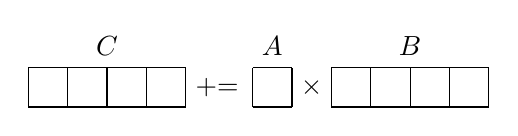
\begin{tikzpicture}[scale=1/2]
      \node[above=.75] at (2, 1) {$C$};
      \draw[shift={(0,0)}] (0,0) grid +(4,1);
      \node at (4.8,.5) {$\mathrel{+}=$};
      \node[above=.75] at (6.2, 1) {$A$};
      \draw[shift={(5.7,0)}] (0,0) grid +(1,1);
      \node at (7.2,.5) {$\times$};
      \node[above=.75] at (9.7, 1) {$B$};
      \draw[shift={(7.7,0)}] (0,0) grid +(4,1);
    \end{tikzpicture}
    \caption{Block times panel mathematically.}
    \label{fig:gebpMath}
  \end{subfigure}
  \hfill
  \begin{subfigure}{.45\linewidth}
    \centering
    \begin{tikzpicture}
      \draw[step=0.8cm,shift={(0,0)}] (0,0) grid +(.8cm,3.2cm);
      \matrix[matrix of nodes,matrix anchor=south west,inner sep=0pt,minimum height=.8cm,text width=.8cm,align=center,shift={(0,0)}]
      {
        $c_{0,0}$\\
        $c_{0,1}$\\
        $c_{0,2}$\\
        $c_{0,3}$\\
      };
      \node at (1.175cm, 1.6cm) {$\mathrel{+}=$};
      \draw[step=0.8cm,shift={(1.6cm,0)}] (0,0) grid +(.8cm,3.2cm);
      \matrix[matrix of nodes,matrix anchor=south west,inner sep=0pt,minimum height=.8cm,text width=.8cm,align=center,shift={(1.6cm,0)}]
      {
        $a_{0,0}$\\
        $a_{0,0}$\\
        $a_{0,0}$\\
        $a_{0,0}$\\
      };
      \node at (2.75, 1.6cm) {$\times$};
      \draw[step=0.8cm,shift={(3.1cm,0)}] (0,0) grid +(.8cm,3.2cm);
      \matrix[matrix of nodes,matrix anchor=south west,inner sep=0pt,minimum height=.8cm,text width=.8cm,align=center,shift={(3.1cm,0)}]
      {
        $b_{0,0}$\\
        $b_{0,1}$\\
        $b_{0,2}$\\
        $b_{0,3}$\\
      };
    \end{tikzpicture}
    \caption{Block times panel in register using \gls{simd} \acrshort{fma}.}
    \label{fig:gebpSimd}
  \end{subfigure}
  \hfill
  \caption[Block and panel kernel mathematically and in register]{Block times panel computation both mathematically and as computed by \glslink{broadcast}{broadcasting} and \acrshort{fma}.\bk{Better caption?}}
  \label{fig:gebp}
\end{figure}

\begin{figure}[t]
  \hfill
  \begin{subfigure}{.45\linewidth}
    \centering
    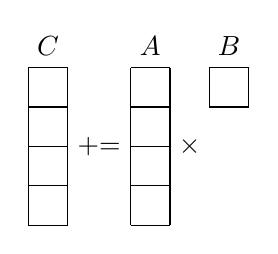
\begin{tikzpicture}[scale=1/2]
      \node[above=.75] at (.5, 4) {$C$};
      \draw[shift={(0,0)}] (0,0) grid +(1,4);
      \node at (1.8,2) {$\mathrel{+}=$};
      \node[above=.75] at (3.1, 4) {$A$};
      \draw[shift={(2.6,0)}] (0,0) grid +(1,4);
      \node at (4.1,2) {$\times$};
      \node[above=.75] at (5.1, 4) {$B$};
      \draw[shift={(4.6,3)}] (0,0) grid +(1,1);
    \end{tikzpicture}
    \caption{Panel times block mathematically.}
    \label{fig:gepbMath}
  \end{subfigure}
  \hfill
  \begin{subfigure}{.45\linewidth}
    \centering
    \begin{tikzpicture}
      \draw[step=0.8cm,shift={(0,0)}] (0,0) grid +(.8cm,3.2cm);
      \matrix[matrix of nodes,matrix anchor=south west,inner sep=0pt,minimum height=.8cm,text width=.8cm,align=center,shift={(0,0)}]
      {
        $c_{0,0}$\\
        $c_{1,0}$\\
        $c_{2,0}$\\
        $c_{3,0}$\\
      };
      \node at (1.175cm, 1.6cm) {$\mathrel{+}=$};
      \draw[step=0.8cm,shift={(1.6cm,0)}] (0,0) grid +(.8cm,3.2cm);
      \matrix[matrix of nodes,matrix anchor=south west,inner sep=0pt,minimum height=.8cm,text width=.8cm,align=center,shift={(1.6cm,0)}]
      {
        $a_{0,0}$\\
        $a_{1,0}$\\
        $a_{2,0}$\\
        $a_{3,0}$\\
      };
      \node at (2.75, 1.6cm) {$\times$};
      \draw[step=0.8cm,shift={(3.1cm,0)}] (0,0) grid +(.8cm,3.2cm);
      \matrix[matrix of nodes,matrix anchor=south west,inner sep=0pt,minimum height=.8cm,text width=.8cm,align=center,shift={(3.1cm,0)}]
      {
        $b_{0,0}$\\
        $b_{0,0}$\\
        $b_{0,0}$\\
        $b_{0,0}$\\
      };
    \end{tikzpicture}
    \caption{Panel times block in register using \gls{simd} \acrshort{fma}.}
    \label{fig:gepbSimd}
  \end{subfigure}
  \hfill
  \caption[Panel and block kernel mathematically and in register]{Panel times block computation both mathematically and as computed by \glslink{broadcast}{broadcasting} and \acrshort{fma}.\bk{Better caption?}}
  \label{fig:gepb}
  \vspace{-0.15cm}
\end{figure}

\bk{
  I'm considering reordering the figures such that \rfig{gebpMath} and \rfig{gepbMath} are together since they're both referenced in one subsection.
  Likewise, \rfig{gebpSimd} and \rfig{gepbSimd} would be together because they're referenced in the next subsection.
  At the same time though, seeing the SIMD implementation with elements is easier if it's grouped with its mathematical representation.
  Thoughts?
}

Goto and van de Geijn's methodology continues to be present within the inner kernel of libraries.
As in the outer kernel, rather than implementing matrix multiplication in terms of the dot product, which some \glspl{isa} have directly supported for years\footnotemark, it is implemented using the multiplication of a combination of a block and a panel.
\footnotetext{For example, the DPPS or DPPD instructions in x86 SSE 4.1 since 2008.}
While for the outer kernel a short dimension is optimally several hundred elements wide and a long dimension is the full extent of one of the matrix dimensions, the inner kernel must operate with registers.
Therefore, a ``short'' dimension is typically a single element and a ``long'' dimension is the length of the vector register.
\rfig{gebpMath} and \rfig{gepbMath} show, in the mathematical sense, what both combinations of block and panel multiplication look like if a vector register can hold four elements.

Next is a discussion of the typical library implementation of these concepts using \gls{simd} techniques in a simple but flawed outer-product.
Following this is a presentation of a method of resolving these flaws through an improved version of the outer product.

\subsubsection{Emulating Outer-Product with \gls{simd} instructions in Libraries}
\rfig{gebpSimd} and \rfig{gepbSimd} show how this is computed using an architecture's \gls{simd} capabilties.
First, the block's single element is \glslink{broadcast}{broadcasted} to each \gls{lane} of a vector register.
The elements of the panel are then loaded into a different vector register.
Once both registers are ready, \ifglsused{fma}{an}{a} \gls{fma} instruction multiplies the two vector registers together and accumulates the result into a third vector register representing a panel in $C$.
This process is more effective than using the dot product because multiple output values are accumulated at the same time in each \gls{lane} of the vector.
However, in a kernel that is supposed to be as tight as possible, cycles are lost to duplicating values.
Furthermore, the kernel should also use resources as effectively as possible, however, the duplicated values use all \glspl{lane} of a vector, effectively reducing a vector registers back to a single scalar, nullifying the benefits of \gls{simd}.

\subsubsection{Improving the Design}
\begin{figure}[t]
  \hfill
  \begin{subfigure}{.40\linewidth}
    \centering
    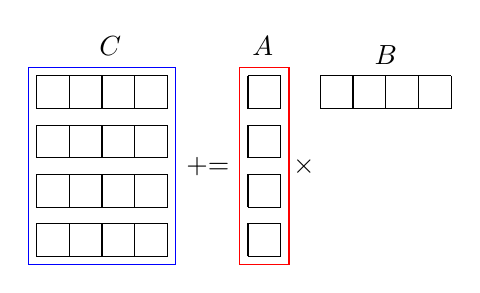
\begin{tikzpicture}[scale=5/12]
      \node[above=.75] at (2, 5.75) {$C$};
      \draw[shift={(-.25,0)}] (0,0) grid +(4,1);
      \draw[shift={(-.25,1.5)}] (0,0) grid +(4,1);
      \draw[shift={(-.25,3)}] (0,0) grid +(4,1);
      \draw[shift={(-.25,4.5)}] (0,0) grid +(4,1);
      \draw[shift={(-.5,-.25)},color=blue] (0, 0) -- +(4.5, 0) -- +(4.5, 6) -- +(0, 6) -- cycle;
      \node at (4.975,2.75) {$\mathrel{+}=$};
      \node[above=.75] at (6.65, 5.75) {$A$};
      \draw[shift={(6.2,0)}] (0,0) grid +(1,1);
      \draw[shift={(6.2,1.5)}] (0,0) grid +(1,1);
      \draw[shift={(6.2,3)}] (0,0) grid +(1,1);
      \draw[shift={(6.2,4.5)}] (0,0) grid +(1,1);
      \draw[shift={(5.95,-.25)},color=red] (0, 0) -- +(1.5, 0) -- +(1.5, 6) -- +(0, 6) -- cycle;
      \node at (7.9,2.75) {$\times$};
      \node[above=.75] at (10.4, 5.5) {$B$};
      \draw[shift={(8.4,4.5)}] (0,0) grid +(4,1);
    \end{tikzpicture}
    \caption{Extending block times panel.}
    \label{fig:extGebp}
  \end{subfigure}
  \hfill
  \begin{subfigure}{.5\linewidth}
    \centering
    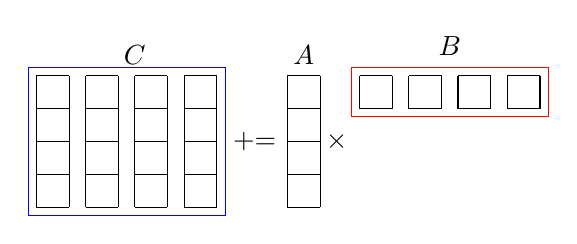
\begin{tikzpicture}[scale=5/12]
      \node[above=.75] at (2.75, 4) {$C$};
      \draw[shift={(-.25,0)}] (0,0) grid +(1,4);
      \draw[shift={(1.25,0)}] (0,0) grid +(1,4);
      \draw[shift={(2.74,0)}] (0,0) grid +(1,4);
      \draw[shift={(4.25,0)}] (0,0) grid +(1,4);
      \draw[shift={(-.5,-.25)},color=blue] (0, 0) -- +(6, 0) -- +(6, 4.5) -- +(0, 4.5) -- cycle;
      \node at (6.4,2) {$\mathrel{+}=$};
      \node[above=.75] at (7.9, 4) {$A$};
      \draw[shift={(7.4,0)}] (0,0) grid +(1,4);
      \node at (8.9,2) {$\times$};
      \node[above=.75] at (12.35, 4.25) {$B$};
      \draw[shift={(9.6,3)}] (0,0) grid +(1,1);
      \draw[shift={(11.1,3)}] (0,0) grid +(1,1);
      \draw[shift={(12.6,3)}] (0,0) grid +(1,1);
      \draw[shift={(14.1,3)}] (0,0) grid +(1,1);
      \draw[shift={(9.35,2.75)},color=red] (0, 0) -- +(6, 0) -- +(6, 1.5) -- +(0, 1.5) -- cycle;
    \end{tikzpicture}
    \caption{Extending panel times block.}
    \label{fig:extGepb}
  \end{subfigure}
  \hfill
  \caption[Extending inner kernels to outer product]{Extending Goto and van de Geijn's inner kernel techniques to outer product.}
  \label{fig:extGoto}
\end{figure}

To improve upon this design, it must first be reexamined.
In choosing this method, the implementer is performing a \matmul{1}{1}{n} or \matmul{n}{1}{1} matrix multiplication.
While it is tempting to view this operation as a traditional inner-product, a different point of view can be more beneficial.
Instead, this multiplication can be regarded as a degenerate case of an outer product where one of the operand vector's length is one.
With this understanding, the direction for improvement becomes apparent.
The duplication issue can be resolved by replacing the duplicated values with unique values, extending the outer product's shortened dimension, bringing it closer to \rfig{outerProduct}.
Doing so stacks more of these operations, as shown in \rfig{extGoto}.
A red box represents one vector register, with each element therein being a distinct element from the matrix rather than a single \glslink{broadcast}{broadcasted} element.
Given a register that could contain the much larger output data in the blue boxes, the overhead of broadcasting can be completely removed and the computational throughput of the operation quadrupled.
\rcha{mma} shows how this is possible using \gls{power10}'s \gls{mma}.

\subsection{Implementation}
\bk{
  This section certainly repeats some previously discussed material.
  My hope is that in discussing it a second time, slightly more in depth, that it reinforces ideas instead of just being redundant.
  If you think it's redundant, please let me know.
}
As discussed previously, libraries often have kernels handwritten in assembly.
Kernel writers must implement all of these optimisations by hand.
In doing so, they must review \gls{cpu} properties as well as consider the design of their outer kernel to determine to what degree an optimisation will affect the hardware.
Historically, with great effort, this process has produced excellent results.

However, all of these optimisations, and others, are readily available in a compiler, often implemented generically and with great care regarding applicability and benefit analysis.
\bk{
  There's an example here that the default vectorisation lowering actually outputs a scalar version of matmul (simpler and easier to reason about/write) that's automatically vectorised by the compiler.
  However, I don't know that I can easily include it because it's based on intrinsics, lowerings, etc. that aren't explained until the method chapter.
}
Therefore, a kernel written within the compiler can be written at a higher and more generic level, as in an \gls{ir}, and achieve the same, or better, performance.
\bk{Section unfinished, got distracted by writing the previous section.}

\section{Usage cases}
\bk{
  Section to be removed per suggestion by Jo\~ao to link usage/motivation earlier.
  Leaving it as a reminder to do so.
}

\end{document}
